
\chapter{抗干扰技术}

所谓干扰,就是各种噪声或造成计算机系统、设备不能正常工作的破坏因素。
干扰在工业现场普遍存在,影响系统的可靠性和稳定性,给系统调试和运行增加了难度。
要做到抗干扰,就要首先了解干扰的来源、传播途径和作用形式。




\section{干扰的来源和传播途径}


\subsection{干扰的来源}

微机控制系统所受到的干扰源分为外部干扰和内部干扰。从机理上看,内外部干扰物理性质相同,因而消除或抑制方法没有本质上的区别


\begin{description}
  \item[外部干扰]
       外部干扰的主要有:分为三类,即电源干扰、空间干扰、设备干扰。
  \item[内部干扰]
       内部干扰主要有:分布电容或分布电感产生的干扰、多点接地造成的电位差给系统带来的影响等。
\end{description}



\subsection{干扰的作用途径}


\begin{description}
  \item[静电耦合]
  干扰信号通过分布电容进行传递称为静电耦合。系统内部各导线之间,印刷线路板的各线条之间,变压器线匝之间的绕组之间以及元件之间、元件与导线之间都存在着分布电容。具有一定频率的干扰信号通过这些分布电容提供的电抗通道穿行,对系统形成干扰。

\begin{figure}[h]
  \centering
  % Requires \usepackage{graphicx}
  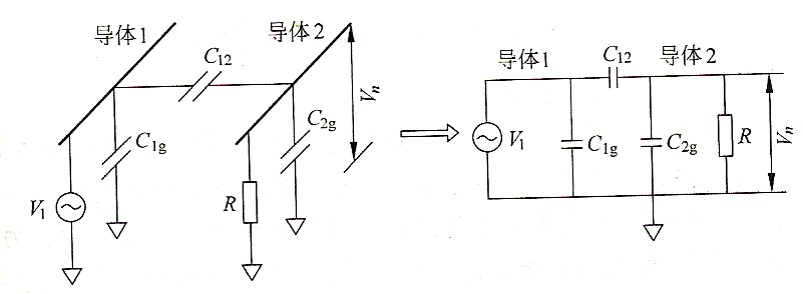
\includegraphics[height=4cm]{fig_4_01.jpg}\\
  \caption{电容耦合}\label{fig_4_01}
\end{figure}

\begin{remark}
对于图\ref{fig_4_01}
\begin{equation}
  V_n=\frac{j\omega RC_{12}}{1+j\omega R(C_{12}+C_{2g})}V_1
\end{equation}
式中起决定作用的是$R$, $C_{12}$, $C_{2g}$和频率$\omega$。分两种情况考虑频率影响:
\begin{equation}
\omega\downarrow\Rightarrow j\omega R(C_{12}+C_{2g})\ll 1 \Rightarrow V_n\ll V_1
\end{equation}
\begin{equation}
\omega\uparrow\Rightarrow j\omega RC_{12}\gg 1 \Rightarrow V_n\approx \frac{
C_{12}}{C_{12}+C_{2g}}V_1
\end{equation}
同样,式中的其它参数也会对结果产生重要影响。
\end{remark}



  \item[电磁耦合]
  电磁耦合是指在空间磁场中电路之间的互感耦合。因为任何载流导体都会在周围的空间产生磁场,而交变磁场又会在周围的闭合电路中产生感应电势,所以这种电磁耦合总是存在的,只是程度强弱不同而已。


\begin{figure}[h]
  \centering
  % Requires \usepackage{graphicx}
  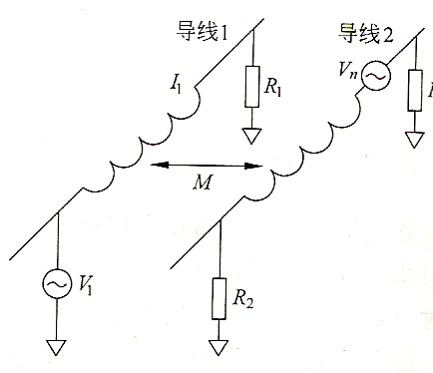
\includegraphics[height=4cm]{fig_4_02.jpg}\\
  \caption{电感耦合}\label{fig_4_02}
\end{figure}

\begin{remark}
对于图\ref{fig_4_02}
\begin{equation}
  V_n=j\omega MI_1
\end{equation}
天津广播电台的地址是和平区卫津路143号,与天津大学相望。大功率广播电台会有较强的电磁辐射,对精密仪器电路产生影响。
\end{remark}

\begin{remark}
叠加定理:在线性电路中,任一支路的电压与电流,都是各个独立源单独作用下,在该支路中产生的电压与电流的代数之和。
\end{remark}

  \item[公共阻抗耦合]
  公共阻抗耦合是指多个电路的电流流经同一公共阻抗时所产生的相互影响。例如系统中往往是多个电路共用一个电源,各电路的电流都流经电源内阻和线路电阻,成为各电路的公共阻抗。每一个电路的电流在公共阻抗上造成的压降都将成为其它电路的干扰信号。

\begin{figure}[h]
  \centering
  % Requires \usepackage{graphicx}
  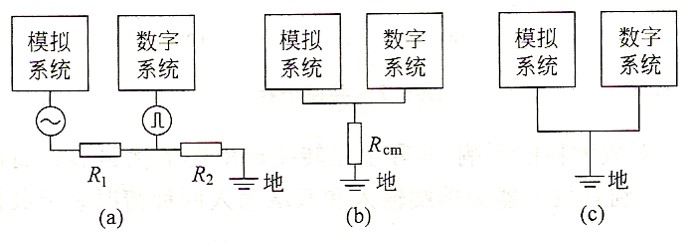
\includegraphics[height=4cm]{fig_4_03.jpg}\\
  \caption{公共阻抗耦合}\label{fig_4_03}
\end{figure}

\begin{remark}
汇流线路不可能是理想的导线($R=0, L=0, C=\infty $)。
如果数字电路与模拟电路部分不是分别接地,则数字电路中的高频信号会通过公共阻抗耦合到模拟电路部分,如图\ref{fig_4_03}(a,b)所示。因而,一般电路中二者分别接地,如图\ref{fig_4_03}(c)所示。
\end{remark}

\end{description}





\subsection{干扰的作用形式 }

各种干扰信号通过不同的耦合方式进入系统后,按照对系统的作用形式又可分为共模干扰、串模干扰和长线传输干扰。
\begin{description}
  \item[共模干扰]
  共模干扰是在电路输入端相对公共接地点同时出现的干扰,也称为共态干扰、对地干扰、纵向干扰、同向干扰等。共模干扰主要是由电源的地、放大器的地以及信号源的地之间的传输线上电压降造成的,如图\ref{fig_4_04}所示。
  \begin{figure}[h]
  \centering
  % Requires \usepackage{graphicx}
  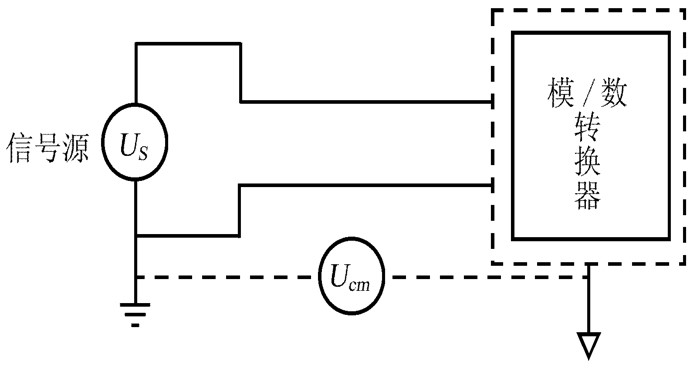
\includegraphics[height=4cm]{fig_4_04.jpg}\\
  \caption{共模干扰}\label{fig_4_04}
\end{figure}



\begin{figure}[h]
  \centering
  % Requires \usepackage{graphicx}
  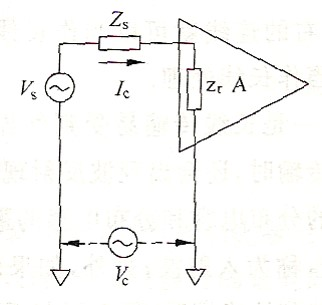
\includegraphics[height=4cm]{fig_4_05.jpg}(a)
  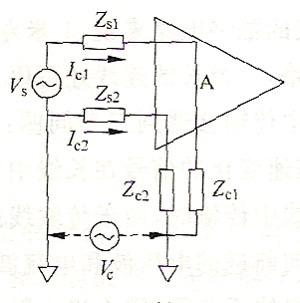
\includegraphics[height=4cm]{fig_4_06.jpg}(b)\\
  \caption{共模干扰的作用形式,(a) 单端输入, (b) 双端输入.}\label{fig_4_05}
\end{figure}


\begin{remark}
共模电压对放大器的影响,实际上是转换成串模干扰的形式而加入到放大器的输入端。

当放大器为单端输入时,如图\ref{fig_4_05}(a) 所示,共模电压Vc 引入放大器输入端的串模干扰电压为:
\begin{equation}
  V_{n1}=I_cZ_s = \frac{Z_s}{Z_s+Z_r}V_c
\end{equation}
其中,$Z_s$ 为信号源内阻;$Z_c$ 放大器输入阻抗。

因为$Z_r\gg Z_s$,得到:
\begin{equation}
  V_{n1}\approx \frac{Z_s}{Z_r}V_c
\end{equation}

如图\ref{fig_4_05}(b) 所示,当放大器为双端输入时,共模电压引入放大器输入端的串模干扰电压为:
\begin{equation}
  V_{n2} = I_{c1}Z_{s1} - I_{c2}Z_{s2} = V_cZ_{s1}/(Z_{s1}+Z_{r1}) - V_{c}Z_{s2}/ (Z_{s2}+Z_{r2})
\end{equation}
其中,Zs1、Zs2为信号源内阻;Zc1、Zc2 为放大器输入端对地的漏阻抗。

因为$Z_{c1} \gg Z_{s1}$, $Z_{c2}\gg Z_{s2}$,

所以$V_{n2} \approx V_c( Z_{s1} / Z_{c1} - Z_{s2} / Z_{c2} )$

当 $Z_{s1} / Z_{c1} = Z_{s2} / Z_{c2}$时,有$V_{n2} = 0$

\end{remark}



  \item[串模干扰]��
  串模干扰就是指串联叠加在工作信号上的干扰,也称之为正态干扰、常态干扰、横向干扰等。
  \item[长线传输干扰]��
  所谓“长线”,取决于集成电路的运算速度。例如,对于毫微秒级的数字电路来说,1米左右的连线就可以当作长线。
  长线传输的三个问题:一是长线传输易受到外界干扰,二是具有信号延时,三是高速变化的信号在长线传输时,还会出现波反射现象。
\end{description}




\section{硬件抗干扰技术}

针对前述噪声的三种作用形式,给出相应的抑制方法。

\subsection{共模干扰的抑制}
抑制共模干扰的主要方法是设法消除不同接地点之间的电位差。
\begin{description}
  \item[变压器隔离] 如图\ref{fig_4_07}所示,利用变压器把模拟电路与数字电路隔离开,也就是把模拟地与数字地断开,以使共模干扰电压无法构成回路,从而抑制共模干扰。注意:隔离变压器的前端和后端电路应当分别采用两组互相独立的电源,切断两部分的地线联系。
\begin{figure}[h]
  \centering
  % Requires \usepackage{graphicx}
  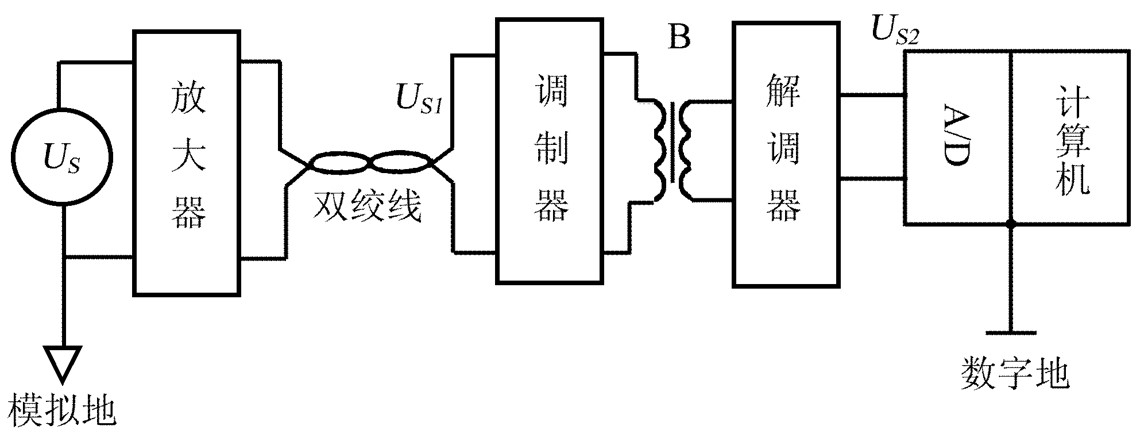
\includegraphics[width=0.4\textwidth]{fig_4_07.jpg}\\(a)\\
  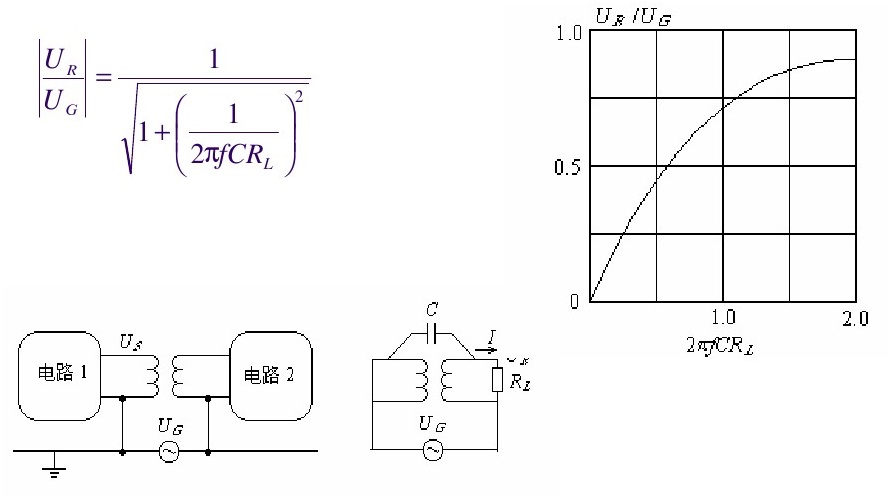
\includegraphics[width=0.6\textwidth]{fig_4_07a.jpg}\\(b)\\
  \caption{变压器隔离}\label{fig_4_07}
\end{figure}

\begin{remark}
变压器隔离可以提供主边到副边之间的隔离,对直流的隔离效果尤其明显。其作用体现在:
\begin{enumerate}
  \item 隔离接地环路;
  \item 电路单元间传输的信号电流只在变压器绕组连线内流过,不流经地线,因此也可以避免对其他电路的干扰。
\end{enumerate}


\end{remark}

  \item[光电隔离]
  如图\ref{fig_4_08}所示,模拟信号经放大后,再利用光电隔离的线性区,直接对模拟信号进行光电耦合传送。


\begin{figure}[h]
  \centering
  % Requires \usepackage{graphicx}
  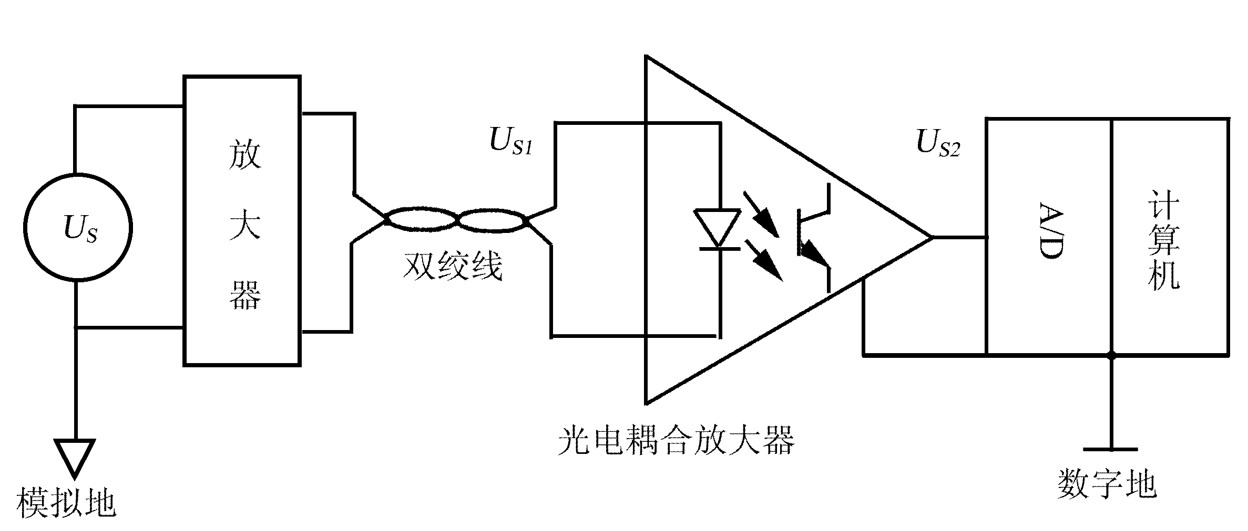
\includegraphics[width=0.4\textwidth]{fig_4_08.jpg}\\
  \caption{光电隔离}\label{fig_4_08}
\end{figure}

  \begin{remark}
  光电耦合具有以下特点:
  \begin{enumerate}
    \item 密封在管壳内,不受外界光的影响;
    \item 靠光传输信号,切断了各电路之间地线的联系;
    \item 其发光二极管只有通过一定的电流时才能发光,从而有效的抑制干扰信号。
  \end{enumerate}
  \end{remark}


  \item[浮地屏蔽]
  采用浮地输入双层屏蔽放大器来抑制共模干扰。所谓浮地,就是利用屏蔽方法使信号的“模拟地”浮空,从而达到抑制共模干扰的目的。
  计算机部分采用内外两层屏蔽,且内屏蔽层对外屏蔽层(机壳地) 是浮地的,而内层与信号源及信号线屏蔽层是在信号端单点接地的,被测信号到控制系统中的放大器是采用双端差动输入方式。

\begin{figure}[h]
  \centering
  % Requires \usepackage{graphicx}
  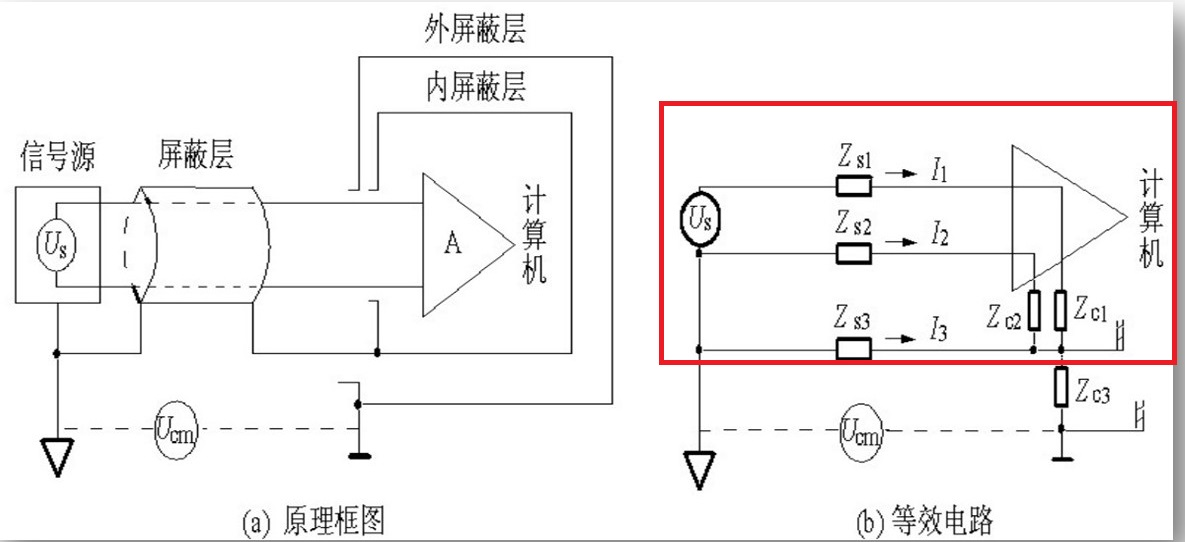
\includegraphics[width=0.6\textwidth]{fig_4_09.jpg}\\
  \caption{浮地屏蔽}\label{fig_4_09}
\end{figure}

  \begin{remark}
  图\ref{fig_4_09}中,Zs1、Zs2为信号源内阻及信号引线电阻,Zs3 为信号线的屏蔽电阻,它们至多只有十几欧姆左右,Zc1、Zc2为放大器输入端对内屏蔽层的漏阻抗,Zc3为内屏蔽层与外屏蔽层之间的漏阻抗。工程设计中Zc1、Zc2、Zc3应达到10兆欧姆以上。
  \end{remark}

  \begin{remark}
  电路分析时,可以分步进行:

  \textbf{第1步}:注意到红线框内的等效电阻Zs 必然满足:$Z_s<Z_{s3}$。 考虑Zs、Zc3与Ucm构成的回路,由于$Z_s \ll Z_{c3}$ ,可知Zs上分得的Ucm信号已被衰减到很小,即
  \begin{equation}
    U_s = U_{cm}\frac{Z_s}{Z_{c3}+Z_s}\ll U_{cm}
  \end{equation}

\textbf{第2步}:可参考对图\ref{fig_4_05}(b) 的分析过程。Us分别在Zs2 与Zs1 上的分压Us2 与Us1 进一步衰减;两个信号加到运放的差动输入端,被再次相减,衰减到很小的共模干扰信号。因而,最终能够进入计算机系统内的共模电压理论上为零。

  \end{remark}

  \item[仪表放大器]
  仪表放大器具有共模抑制能力强、输入阻抗高、漂移低、增益可调等优点,是一种专门用来分离共模干扰与有用信号的器件。
\end{description}

\subsection{串模干扰的抑制}
对于串模干扰的抑制比较困难。
\begin{description}
  \item[滤波]
    如果串模干扰频率比被测信号频率高,则采用输入低通滤波器来抑制高频串模干扰;如果串模干扰频率比被测信号频率低,则采用高通滤波器来抑制低频串模干扰;如果串模干扰频率落在被测信号频谱的两侧,应采用带通滤波器。
   一般情况下,串模干扰均比被测信号变化快,故常用二阶阻容低通滤波网络作为模/数转换器的输入滤波器。
  \item[采用双绞线作为信号线]
    若串模干扰和被测信号的频率相当,则很难用滤波的方法消除。此时,必须采用其它措施,消除干扰源。通常可在信号源到计算机之间选用带屏蔽层的双绞线或同轴电缆,并确保接地正确可靠。
    采用双绞线作为信号引线的目的是减少电磁干扰。双绞线能使各个小环路的感应电势相互抵消。一般双绞线的节距越小抗干扰能力越强。

\begin{figure}[h]
  \centering
  % Requires \usepackage{graphicx}
  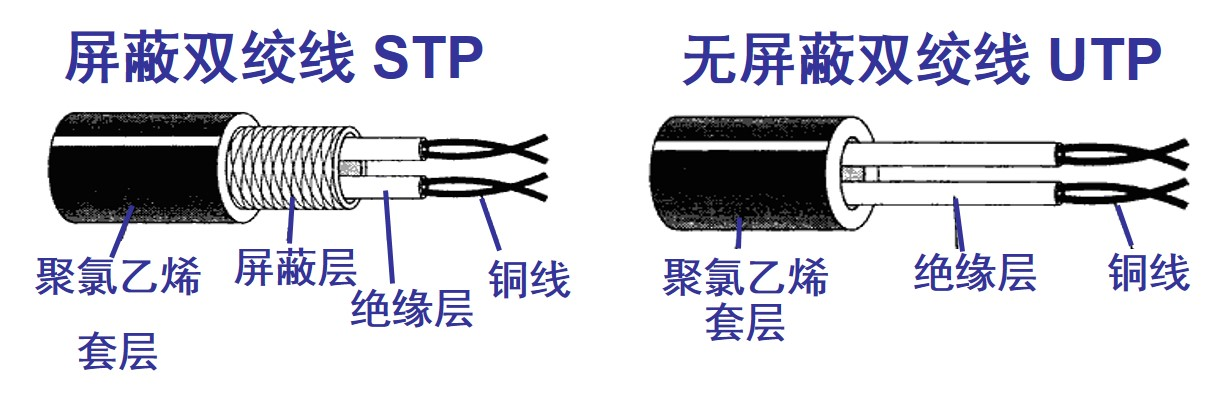
\includegraphics[height=3cm]{fig_4_10.jpg}\\
  \caption{双绞线}\label{fig_4_10}
\end{figure}

\begin{figure}[h]
  \centering
  % Requires \usepackage{graphicx}
  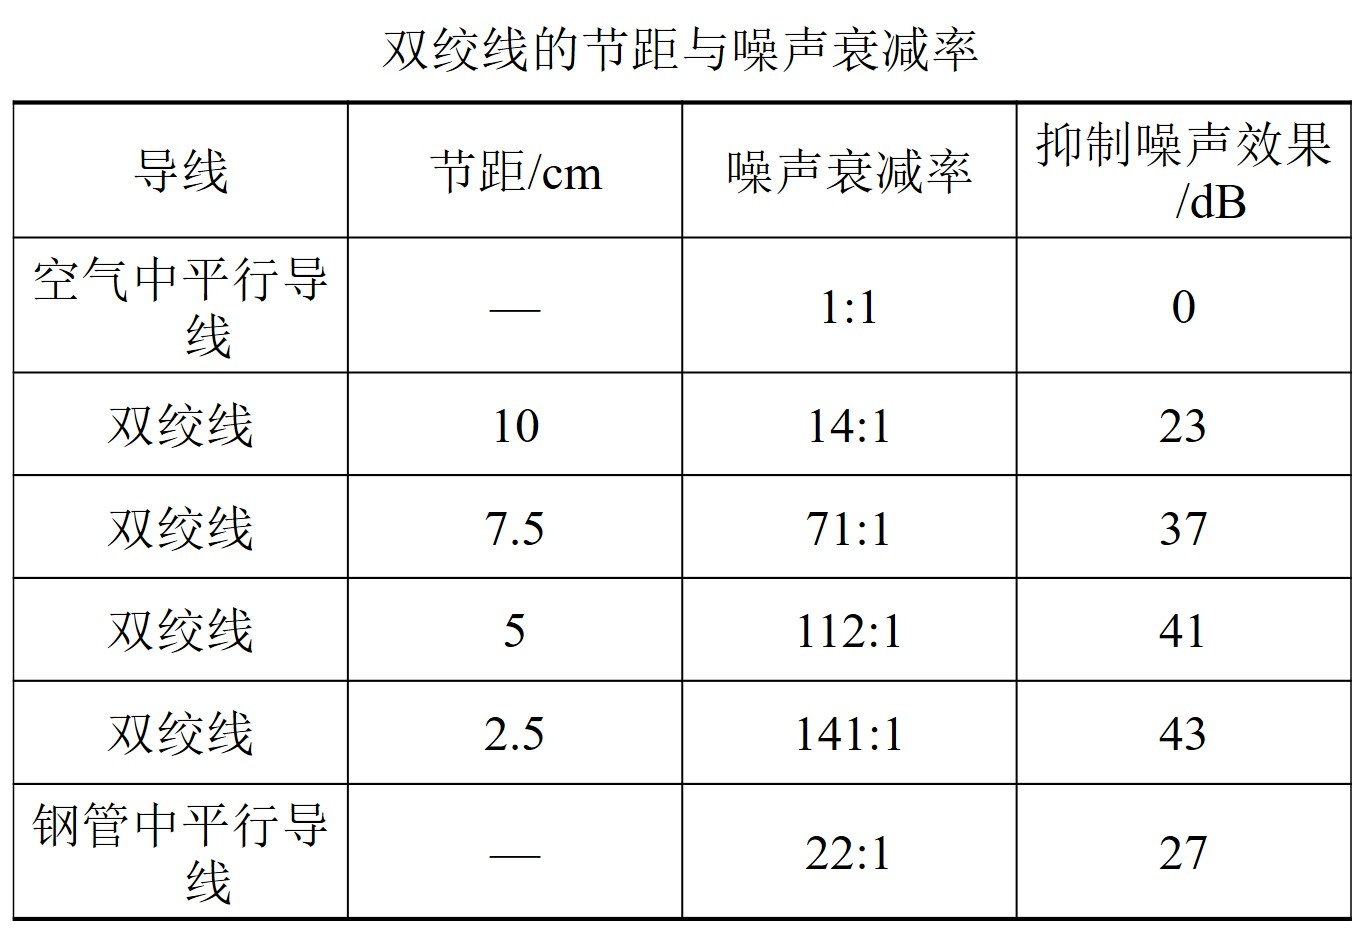
\includegraphics[height=5cm]{fig_4_11.jpg}\\
  \caption{双绞线的节距与噪声衰减率}\label{fig_4_11}
\end{figure}



  \item[电流传送]
    当传感器信号距离主机很远时很容易引入干扰。如果在传感器出口处将被测信号由电压转换为电流,以电流形式传送信号,将大大提高信噪比,从而提高传输过程中的抗干扰能力。
\begin{remark}
\textit{
4-20mA信号指定时考虑了在多方面使用的要求:
\begin{enumerate}
  \item 30V 电压 30mA 电流 所引起的火花是可以点燃危险气体平均下限,为了保险起见,同时参照其它传统设定,所以将许多仪表定为24V供电,同时限定电流小于30mA,为了留有余地,信号上限定为 20mA。
  \item 为了区分没有信号,和信号为零,信号的起始值(信号零位值)不能为零(电气值)。
  \item 两线制仪表在信号值为零时仍需要一定的能量供应,在24V供电条件下,4mA电流提供的能量,是当时制定标准时,大部分仪表生产商能接受的能量供应下限。
  \item 4-20mA电流作用在250欧姆电阻上正好符合标准信号的电压标准 1-5V。
\end{enumerate}
上面几个条件经过整合,形成一套信号标准,包括:
24V直流供电、250欧姆标准负载、1-5V 或 4-20mA 标准信号。}
\end{remark}
\end{description}


\subsection{长线传输干扰的抑制}


采用带有屏蔽的双绞线可以在很大程度上减少空间电磁场的干扰;采用终端阻抗匹配或始端阻抗匹配,可以消除长线传输中的波反射或者把它抑制到最低限度。

\begin{description}
  \item[波阻抗的测量] 为进行阻抗匹配,必先知道长传输线的波阻抗Rp。波阻抗的测量如图\ref{fig_4_12}所示。调节电阻并用示波器观察电路A 的波形,当达到完全匹配时,即R=Rp 时,电路A输出的波形不畸变,反射波完全消失。此时的R为该线的波阻抗。

\begin{remark}
  一般双绞线的波阻抗在100-200欧姆,绞节距愈短,波阻抗愈低。同轴电缆的波阻抗一般在50-100欧姆。根据传输线的基本理论,无损耗导线的波阻抗为
  \begin{equation}
    R_p=\sqrt{\frac{L_0}{C_0}}
  \end{equation}
\end{remark}

\begin{figure}[h]
  \centering
  % Requires \usepackage{graphicx}
  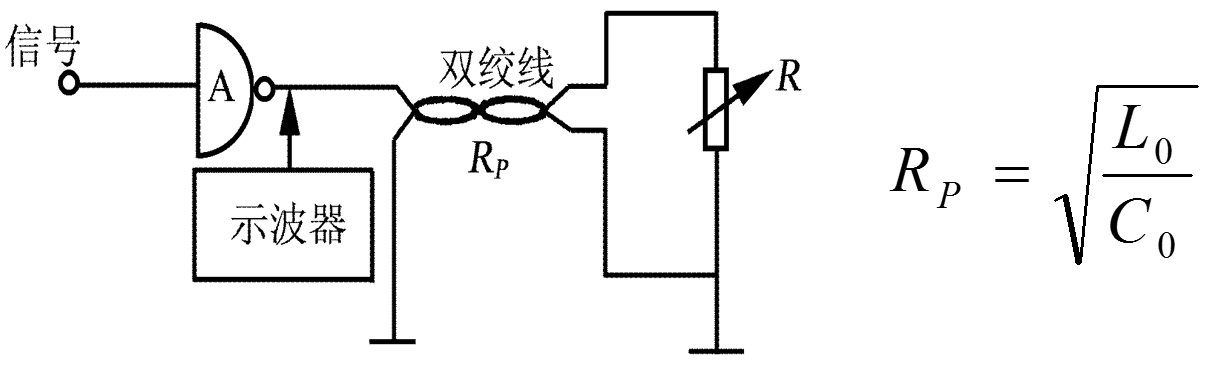
\includegraphics[height=2cm]{fig_4_12.jpg}\\
  \caption{波阻抗的测量}\label{fig_4_12}
\end{figure}
  \item[波阻抗的终端匹配]
  最简单的终端阻抗匹配方法如图\ref{fig_4_13}(a)所示,其中R=Rp。

\begin{figure}[h]
  \centering
  % Requires \usepackage{graphicx}
  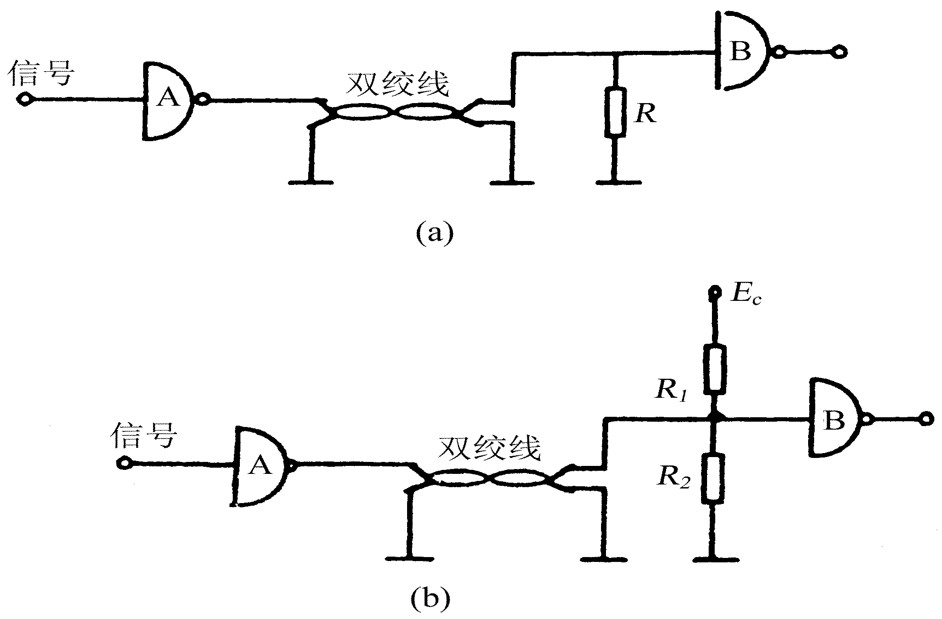
\includegraphics[height=5cm]{fig_4_13.jpg}\\
  \caption{长线传输中波阻抗的终端匹配}\label{fig_4_13}
\end{figure}

  \begin{remark}

由于R的存在加大了负载,使得信号波形电平下降,影响其对高电平的抗干扰能力。为此,可采用图\ref{fig_4_13}(b)所示的方法。注意其等效电阻R为:
\begin{equation}
  R=\frac{R_1R_2}{R_1+R_2}
\end{equation}
使其满足R=Rp。
  \end{remark}

  \item[波阻抗的始端匹配]

  在传输线的始端接入电阻R,也可消除波反射现象,如图\ref{fig_4_14}所示。
\begin{figure}[h]
  \centering
  % Requires \usepackage{graphicx}
  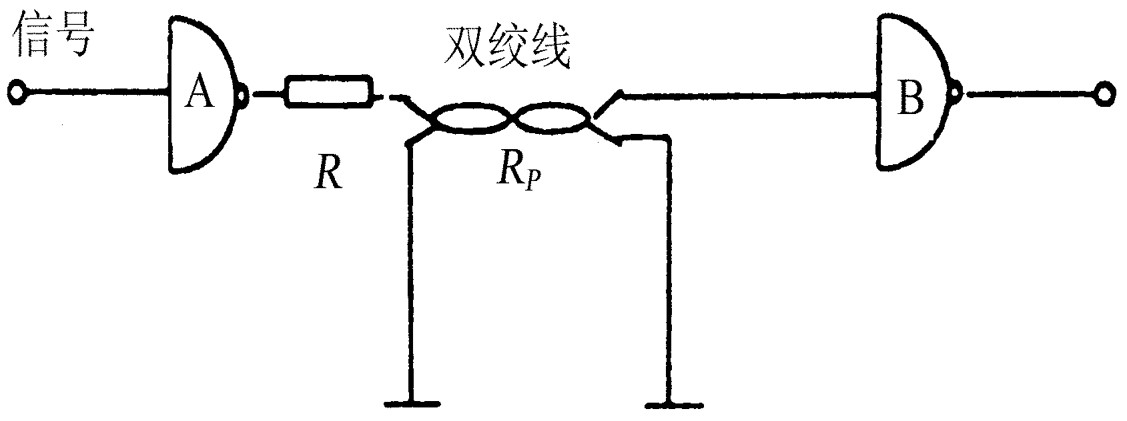
\includegraphics[height=2cm]{fig_4_14.jpg}\\
  \caption{长线传输中波阻抗的始端匹配}\label{fig_4_14}
\end{figure}

\begin{remark}
选择R时应满足:
\begin{equation}
  R=R_p-R_{src}
\end{equation}

\end{remark}


\end{description}


\section{软件抗干扰技术}
\subsection{输入/输出软件抗干扰措施}

\begin{description}
  \item[开关量(数字量)信号输入抗干扰措施]
�ザ杂诳�关量的输入,为了确保信息准确无误,在软件上可采取多次读取的方法(至少读两次),认为无误后再行输入,如图\ref{fig_4_15}示。
\begin{figure}[h]
  \centering
  % Requires \usepackage{graphicx}
  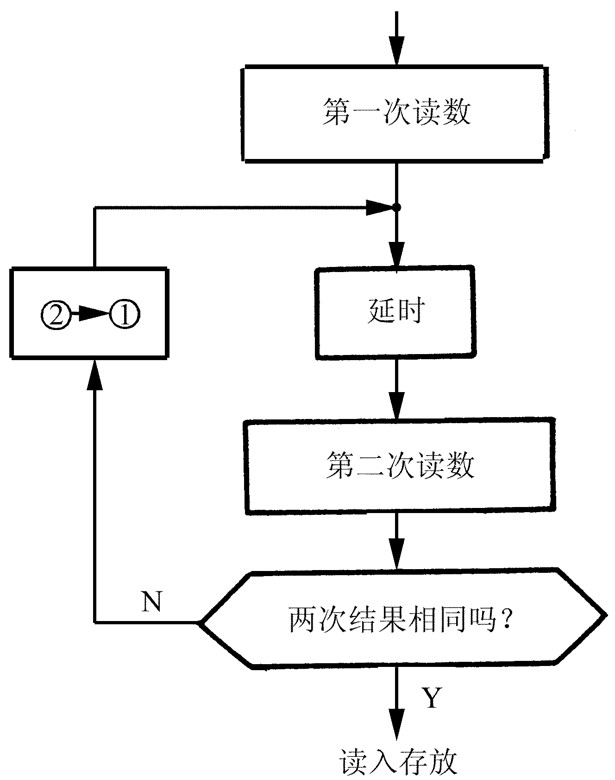
\includegraphics[height=5cm]{fig_4_15.jpg}\\
  \caption{输入抗干扰}\label{fig_4_15}
\end{figure}


  \item[开关量(数字量)信号输出抗干扰措施]     当计算机输出开关量控制闸门、料斗等执行机构动作时,为了防止这些执行机构由于外界干扰而误动作,比如已关的闸门、料斗可能中途打开;已开的闸门、料斗可能中途突然关闭。对于这些误动作,可以在应用程序中每隔一段时间(比如几个ms) 发出一次输出命令,不断地关闭闸门或者开闸门。这样,就可以较好地消除由于扰动而引起的误动作(开或关)。
\end{description}


\begin{remark}

在某个输出口上输出一个高电平去驱动一个外部器件,你如果只送一次“1”,那么,当干扰来临时,这个“1”就有可能变成“0”了。正确的处理方式是,你定期刷新这个“1”。那么,即使偶然受了干扰,它也能恢复回来。除了I/O口动作的冗余。同时也建议大家在下面各方面也采用这种方法:

1、LCD的显示。有时,也许你会用一些LCD的专用驱动芯片(如HT1621),这种芯片有个好处,即你只要将显示数据传送给它,它就会不断的自动扫描LCD。但是,你千万不要以为这样就没你啥事了。正确的处理方式是,要记得定期刷新送显数据(即使显示内容没有改变)。对于CPU中自带LCD DRIVER 的,也要定期刷新LCD RAM。

2、中断使能标志的设置。不要以为你在程序初始化段将中断设置好就OK了。应该在主程序中适当的地方定期刷新一下,以免你的中断被挂起来。

3、其它一些标志字和参数寄存器(包括你自己定义的),也要记得常常刷新。

4、其它一些你认为有必要的地方。
\end{remark}


\subsection{软件冗余技术}

程序正常运行时,程序计数器PC始终指向正在执行的这条指令的下一条指令的第一个字节的程序存储器单元地址,这样就保证了单片机能够正确地读取每一条指令的各个字节,即CPU先读取操作码,再读取操作数(如果有操作数字节的话)。在MCS51系列单片机中,程序计数器PC的寻址范围是0000H~FFFFH, 共64KB。用户应用程序中,根据系统要求,规定了程序运行的惟一路径。这体现在系统上电后,程序计数器PC有唯一的变化历程,保证了程序正常、有序地运行。程序跑飞是指系统受到某种干扰后,程序计数器PC的值偏离了给定的唯一变化历程,导致程序运行偏离正常的运行路径。程序跑飞因素及后果往往是不可预计的。

在很多情况下,程序跑飞后系统会进入死循环而导致死机。这时,
应采取有效措施引导跑飞的程序尽快退出死循环并迅速复位。实践证明,软件陷阱技术能有效引导跑飞的程序尽快退出死循环并迅速复位。


当单片机应用系统的CPU受到干扰时,不良影响的主要形式有:

\begin{enumerate}
  \item 非正常修改程序计数器PC指针;
  \item 改写可编程输出端口的状态;
  \item 非正常修改重要数据区的数据。
\end{enumerate}

以上三个方面的不良影响会使单片机应用系统程序失控,控制状态失灵,其后果是非常严重的,它甚至会使系统崩溃,造成严重的工业事故。

\begin{description}
  \item[数据冗余]     数据冗余就是将要保护的原始数据在另外两个区域同时存放,建立两个备份,当原始数据块被破坏时,用备份数据块去修复。备份数据的存放地址应远离原始的存放地址以免被同时破坏。数据区也不要靠近栈区,以防止万一堆栈溢出而冲掉数据。
\begin{remark}
  所谓数据冗余,就是:

  1、将重要的数据信息备份2份(或以上)并存放在RAM中不同的区域(指地址不相连)。

  2、当平时对这些数据进行修改时,同时也更新备份。

  3、当干扰发生并被拦截到“程序错误处理段”中时,将数据与备份做比较,采用表决方式(少数服从多数)选出正确(或可能正确?)的那个。

  4、备份越多,效果越好。(当然,你得有足够的存储空间)。

  5、只备份最最原始的数据。中间变量(指那些可以从原始数据重新推导出来的数据)不必备份。

注:

  这种思路的理论依据,源于“概率论”,即所有数据备份同时毁坏的概率是远小于其中任一备份单独损坏的概率。
\end{remark}
  \item[指令冗余]    当CPU受到干扰后,往往将一些操作数当作指令码来执行,引起程序混乱。当程序弹飞到某一单字节指令上时,便自动纳入正轨。当弹飞到某一双字节指令上时,有可能落到其操作数上,从而继续出错。当程序弹飞到三字节指令上时,因它有两个操作数,继续出错的机会更大。因此,我们应多采用单字节指令,并在关键的地方人为地插入一些单字节指令(NOP)或将有效单字节指令重复书写,这便是指令冗余。

\end{description}


\subsection{程序运行失常的软件抗干扰}

\begin{description}
  \item[设置软件陷阱]     当干扰导致程序计数器PC值混乱时,可能造成CPU离开正确的指令顺序而跑飞到非程序区去执行一些无意义地址中的内容,或进入数据区,把数据当作操作码来执行,使整个工作紊乱,系统失控。针对这种情况,可以在非程序区设置陷阱,一旦程序飞到非程序区,很快进入陷阱,然后强迫程序由陷阱进入初始状态。
    所谓软件陷阱,就是一条引导指令,强行将捕获的程序引向一个指定的地址,在那里有一段专门对程序出错处理的程序。

    软件陷阱安排在以下4 种地方:

    \begin{enumerate}
      \item 未使用的中断向量区
      \item 未使用的大片ROM空间
      \item 表格
      \item 程序区
    \end{enumerate}
\begin{remark}
  当CPU受到外界干扰,有时PC指针会飞到另一段程序中,或跳到空白段去。其实,如果PC指针飞到空白段去,倒也好处理。只要在空白段设立软件陷阱(拦截指令),将程序拦截到初始化段或程序错误处理段。

\begin{verbatim}
NOP
NOP
LJMP ERR
\end{verbatim}

\end{remark}

  \item[设置监视跟踪定时器] 也称为看门狗定时器(Watchdog),可以使陷入“死机”的系统产生复位,重新启动程序运行。这是目前用于监视跟踪程序运行是否正常的最有效的方法之一,近来得到了广泛的应用。
    在程序运行的每个循环周期内,对定时器重新初始化。如果程序运行失常,跑飞或进入局部死循环,不能按正常循环路线运行,则Watchdog定时器得不到及时的重新初始化而使定时时间到,引起复位。一般而言,控制程序具备以下基本结构:

\begin{verbatim}
void main()
{
    init();     %初始化
    while(1)
        loop(); %主循环
}
\end{verbatim}



\begin{remark}
程序正常运行时,loop()具有确定的运行周期Ta;而程序出现异常时,loop()的周期性被打乱。由此,可以判断系统程序是否正常。


\end{remark}


\begin{remark}
思考:如何利用这一特点来监控/管理CPU的运行状态呢?



看门狗的主体是一个定时器。其功能为:每隔一定周期Tc产生一个定时器溢出;如在定时器溢出前对其清零,则重新计时。

在loop()中加入指令,可周期性(Ta)的清零看门狗定时器。这一操作,称为“喂狗”。注意:Tc略大于Ta。以下分两种情况分析:

\begin{enumerate}
  \item 当程序正常运行时,loop()中的这一条指令能够定时“喂狗”,则狗儿不叫,定时器不会溢出;
  \item 而当程序出现异常时,loop()中的喂狗指令不会被运行,没有喂狗,则狗儿会叫,定时器会溢出;
\end{enumerate}

定时器溢出,可用于触发对CPU的复位或NMI,使CPU程序能够恢复正常运行。

\end{remark}

\begin{remark}

看门狗可分为硬件看门狗和软件看门狗两种。


软件看门狗原理上一样,只是将硬件电路上的定时器用处理器的内部定时器代替。这样可以简化硬件电路设计,但在可靠性方面不如硬件定时器,比如系统内部定时器自身发生故障就无法检测到。当然也有通过双定时器相互监视,这不仅加大系统开销,也不能解决全部问题,比如中断系统故障导致定时器中断失效。

看门狗本身不是用来解决系统出现的问题,在调试过程中发现的故障应该要查改设计本身的错误。加入看门狗目的是对一些程序潜在错误和恶劣环境干扰等因素导致系统死机而在无人干预情况下自动恢复系统正常工作状态。看门狗也不能完全避免故障造成的损失,毕竟从发现故障到系统复位恢复正常这段时间内是不能正常工作的。同时一些系统也需要复位前保护现场数据,重启后恢复现场数据,这可能也需要一笔软硬件的开销。
\end{remark}

\end{description}

\begin{figure}[h]
  \centering
  % Requires \usepackage{graphicx}
  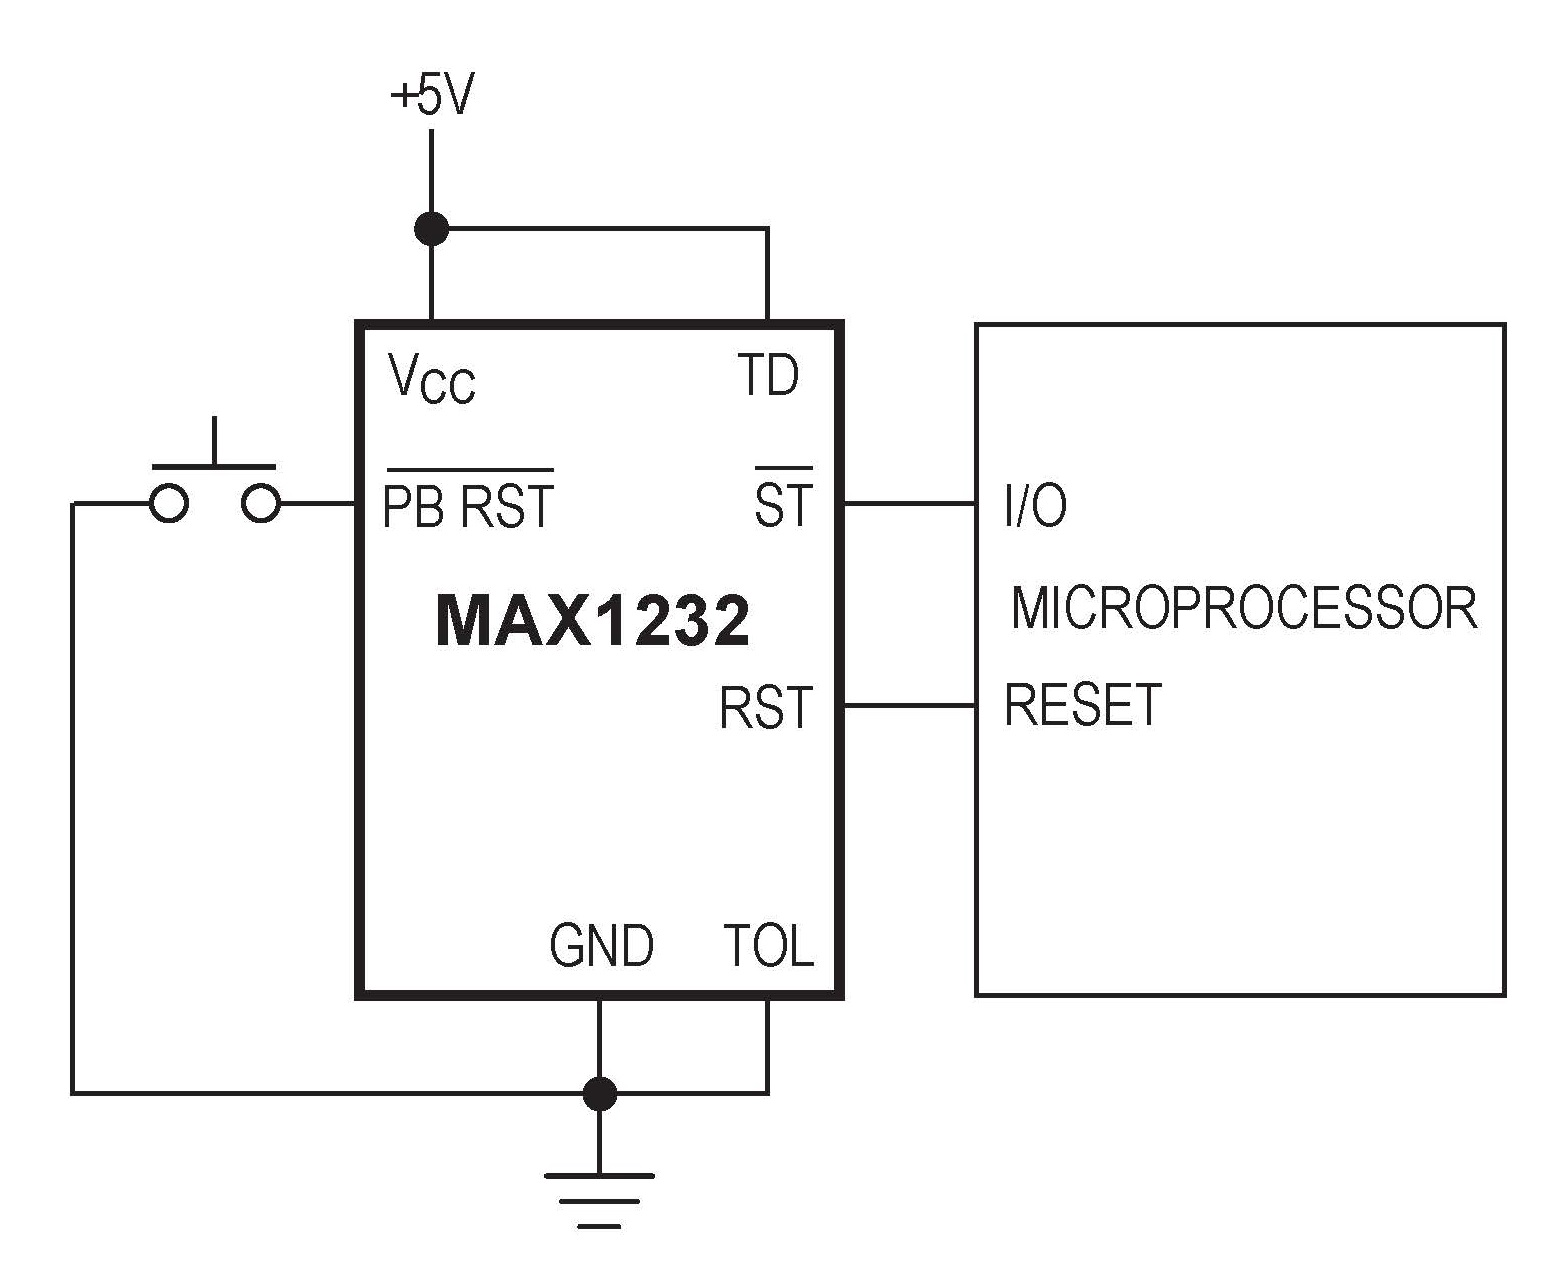
\includegraphics[width=0.4\textwidth]{fig_4_16.jpg}\\
  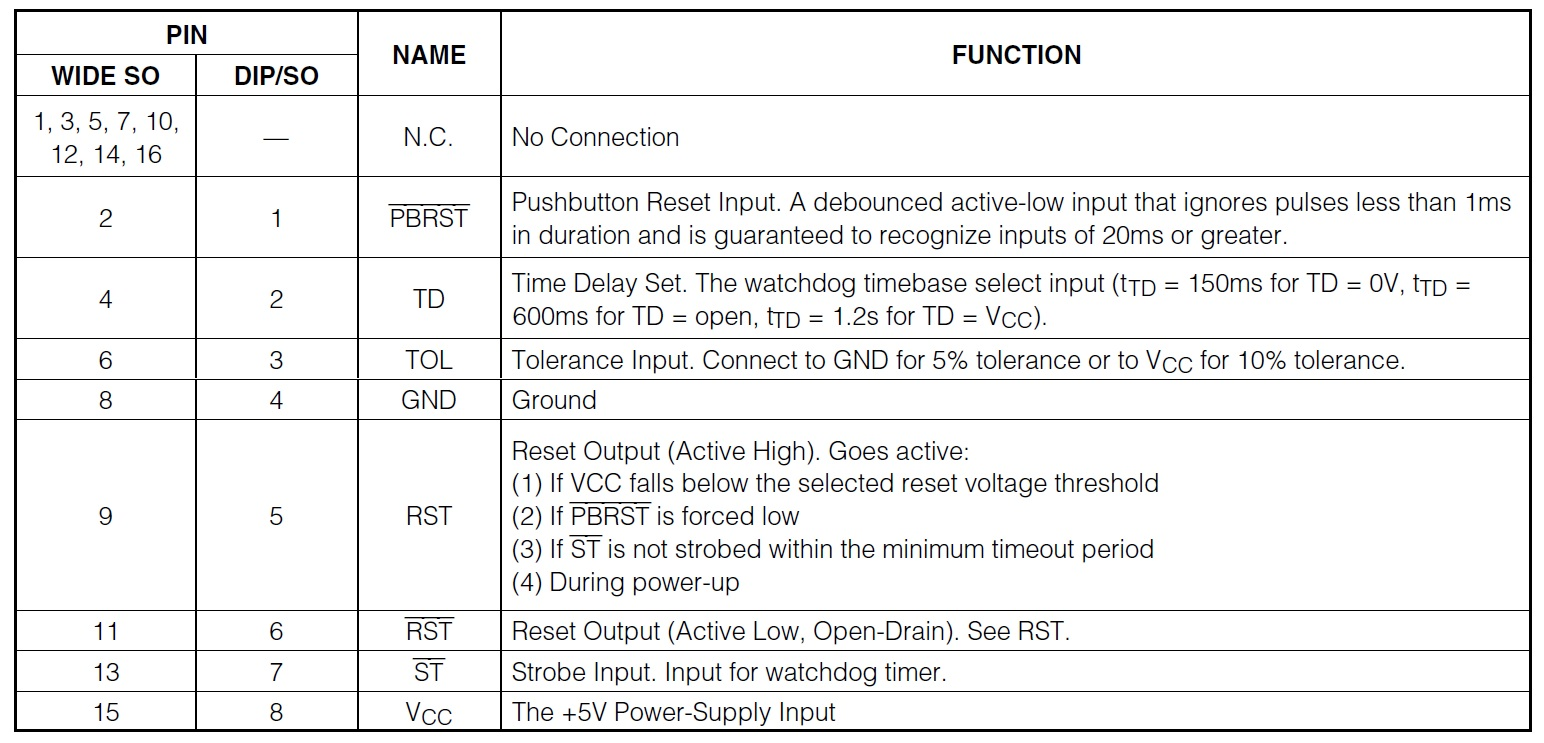
\includegraphics[width=0.7\textwidth]{fig_4_16a.jpg}
  \caption{MAX1232 连接及管脚定义}\label{fig_4_16}
\end{figure}




\subsection{其他手段}

\begin{enumerate}
  \item 分散结构设计

把整体的软件设计分散成各子系统的设计,各自独立,又共享资源。
\item 容错技术

在软件设计中的容错技术是指在软件设计时,对误操作不予响应的技术。基本活动有四种:故障检测、损坏估计、故障恢复和缺陷处理。
\item 标准化

采用标准化的软件可以提高软件运行的可靠性。

\end{enumerate}





\section{供电与接地技术}


\subsection{供电技术}
电网的干扰,频率的波动将直接影响系统的可靠性与稳定性。考虑采取电源保护措施,防止电源干扰,并保证不间断地供电。

\subsubsection{交流电源系统}

供电系统的一般保护,如图\ref{fig_4_17} 所示。

(1)选用供电比较稳定的进线电源;

(2)利用干扰抑制器消除尖峰干扰;

(3)采用交流稳压器稳定电网电源。
\begin{figure}[h]
  \centering
  % Requires \usepackage{graphicx}
  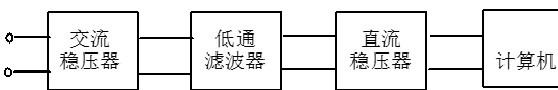
\includegraphics[width=0.5\textwidth]{fig_4_17}\\
  \caption{交流电源系统}\label{fig_4_17}
\end{figure}




\subsubsection{直流电源系统}

供电系统的一般保护,如图\ref{fig_4_18} 所示。

(1)交流电源变压器的屏蔽;

(2)采用直流开关电源;

(3)直流供电系统的隔离。

\begin{figure}[h]
  \centering
  % Requires \usepackage{graphicx}
  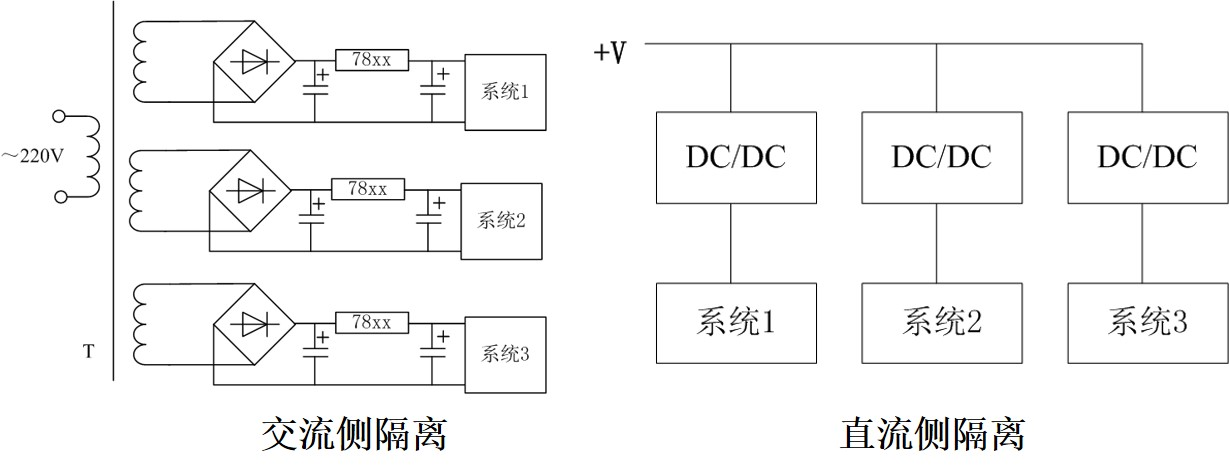
\includegraphics[width=0.6\textwidth]{fig_4_18}\\
  \caption{直流电源系统}\label{fig_4_18}
\end{figure}



\subsection{接地技术}


\subsubsection{地线系统的分析}

  地线的分类:
\begin{enumerate}
\item 模拟地:它是放大器,A/D,D/A转换器中的模拟电路零电位。
\item 数字地:各种数字电路的零电位。
\item 安全地:目的是使设备机壳与大地等电位,以避免机壳带电而影响人身及设备的安全(通常又称为保护地或机壳地);
\item 系统地:上述几种地的最终汇流点,直接与大地相连;
\item 交流地:交流50Hz电源的地线,它是噪声地。
\end{enumerate}


\subsubsection{主机系统的接地}

根据接地理论,低频电路(频率小于1MHz) 应单点接地,高频电路(频率大于10MHz)应就近多点接地。介于低频与高频之间时,单点接地的地线长度不得超过波长的1/20,否则应采用多点接地。


\subsubsection{接地方式}

\begin{enumerate}



\item 单点接地如图\ref{fig_4_19}所示,包括:

\begin{description}
    \item[串联接地] 各电路间相互会发生干扰, 适用各电路的电平相差不大.
    \item[并联接地] 不会因地电流而引起各电路间的耦合,其缺点是需要连很多根地线。
\end{description}


\begin{figure}[h]
  \centering
  % Requires \usepackage{graphicx}
  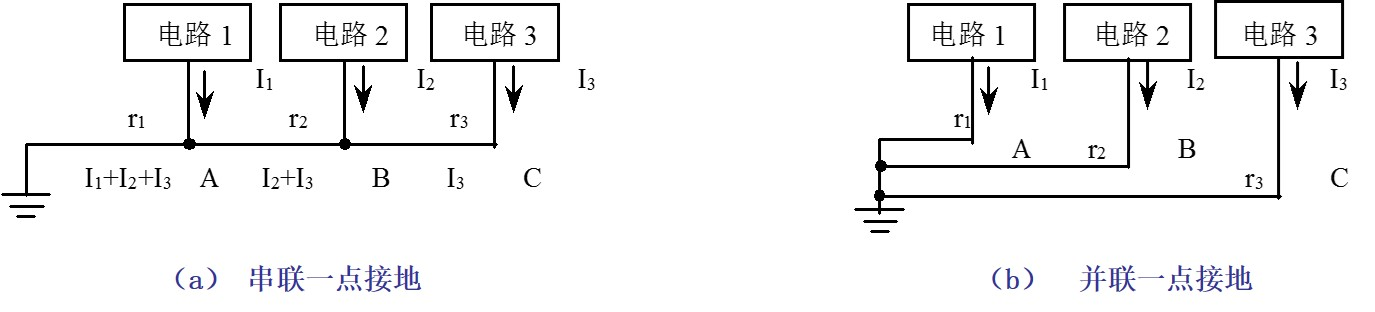
\includegraphics[width=0.6\textwidth]{fig_4_19}\\
  \caption{单点接地}\label{fig_4_19}
\end{figure}


\item 汇流法单点接地,如图\ref{fig_4_20}所示:


\begin{figure}[h]
  \centering
  % Requires \usepackage{graphicx}
  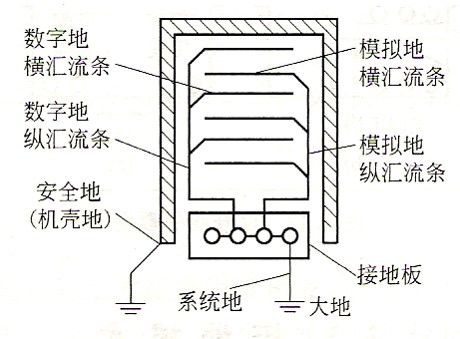
\includegraphics[width=0.35\textwidth]{fig_4_20}\\
  \caption{汇流法接地}\label{fig_4_20}
\end{figure}



\item 输入通道的接地技术,如图\ref{fig_4_21}所示,包括:

\begin{description}
  \item[电路一点地基准]
信号源端接地时,放大器电源不接地;放大器接地时,信号源不接地。
  \item[电缆屏蔽层的接地] 信号电路一点接地时,低频电缆的屏蔽层也一点接地。
\end{description}


\begin{figure}[h]
  \centering
  % Requires \usepackage{graphicx}
  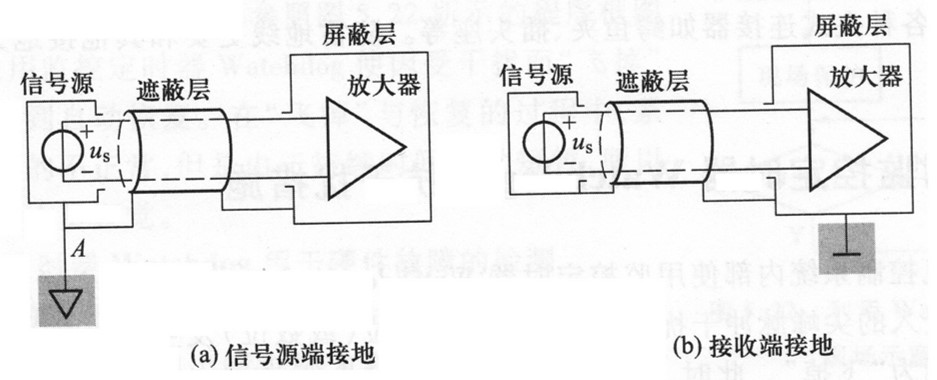
\includegraphics[width=0.5\textwidth]{fig_4_21}\\
  \caption{输入通道的接地}\label{fig_4_21}
\end{figure}

\item 多机一点接地,如图\ref{fig_4_22}(a)所示:

\begin{figure}[h]
  \centering
  % Requires \usepackage{graphicx}
  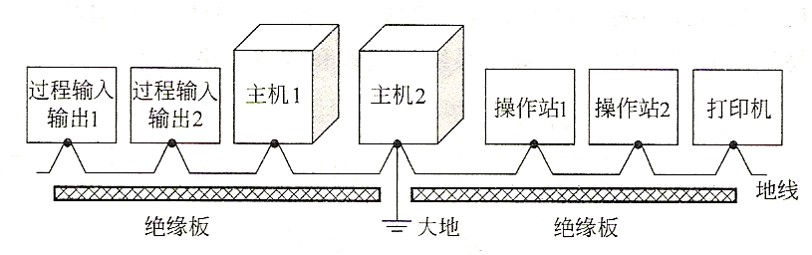
\includegraphics[width=0.5\textwidth]{fig_4_22}(a)
  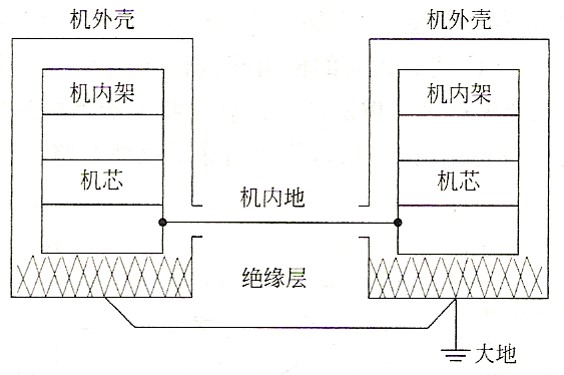
\includegraphics[width=0.3\textwidth]{fig_4_23}(b)\\
  \caption{(a)多机一点接地, (b)主机外壳接地及机芯浮空}\label{fig_4_22}
\end{figure}



\item 主机外壳接地及机芯浮空,如图\ref{fig_4_22}(b)所示:



\end{enumerate}


\section{本章要点总结}

\begin{itemize}

\item 了解干扰的来源和传播途径;
\item 了解硬件抗干扰的常用方法;
\item 了解输入/输出软件抗干扰措施、软件冗余以及程序运行失常的软件抗干扰 ;
\item 了解接地系统以及不同的接地技术;

\end{itemize}
